\section{Description of the model} \label{model}
\subsection{Autoencoders}
Autoencoders are widely used in Deep Learning applications with the main intention
the describe a set of data, mostly targeting dimensionality reduction of creating
a general represenation of the dataset.
This allows the application of such models for anomaly detection, that can be translated
as outlier detection problem in this generated representation,
called feature vector or latent space.
Such approach does not require annotated dataset, therefore belongs to the class of
unsupervised learning algorithms.

The general structure of Autoencoders are shown in Figure \ref{fig:autoencoder}.

\begin{figure}[!ht]
    \centering
    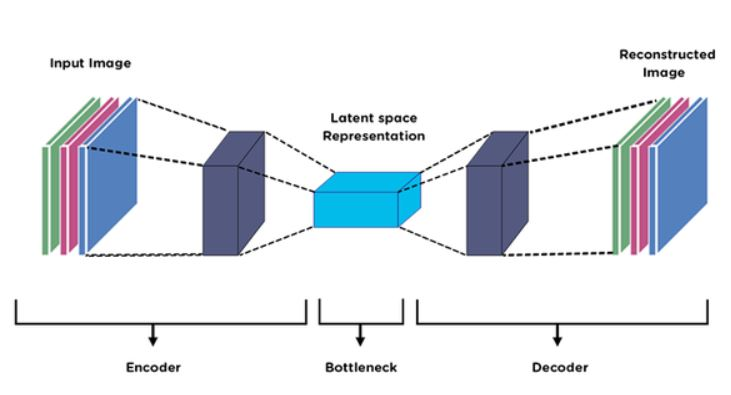
\includegraphics[width=0.6\textwidth]{./tex_images/autoencoder.jpeg}
    \caption{General structure of Autoencoders \cite{khosla_auto_2021}}
    \label{fig:autoencoder}
\end{figure}

The basic idea behind an Autoencoder model is to generate feature vectors from the input
dataset (encode the dataset), this is the so-called Encoder part.
This set of feature vectors, called as latent space contains the represenation of the dataset.
In the second part, the Decoder parts tries to recreate the input data based on the feature vector
generated by the Encoder.
In current use case this means that the single images of the rail is translated to feature vectors
and then the original image is recreated with some error using the Decoder.

A comprehensive overview about Deep Learning methodology is given in \cite{Goodfellow-et-al-2016}.
Chapter 14 of this book explains that mathemathical structure of Autoencoders.
Another introduction can be found at \cite{_autoencoder_2023}.

\subsection{Type of Encoders}
During the research four type of Encoders used as listed below.

\begin{itemize}
    \item VGG19
    \item VGG19 with batch normalization
    \item ResNet50
    \item EfficientNetV2L
\end{itemize}

The VGG19 is one of the first deep convolutional networks introduced in \cite{simonyan_very_2015}.
In the second model batch normalization was added after each convolutional layer.
The ResNet50 \cite{he_deep_2015} overcomes the issue of the wanishing gradient
by adding the skip connections.
EfficientNetV2 \cite{tan_efficientnetv2_2021} is developed to reduce training time
and provide better parameter efficiency than previous models.

During the encoding the input image sizes are gradually reduced in four steps,
resulting different shapes of the latent space due to the different number of filters applied.
An overview of the resulting latent space considering an input size of 704 x 288
is shown in Table \ref{table:latent_space_shape}.
For comparison the original image of size 720 x 288 x 3 has a total number of 622080 to describe
a single instance.

\begin{table}[!ht]
    \centering
    \begin{tabular}{l c c}
        Encoder type                   & Width x Height x Filters & Number of parameters \\
        \hline
        VGG19                          & 22 x 9 x 512             & 101376               \\
        VGG19 with batch normalization & 22 x 9 x 512             & 101376               \\
        Resnet50                       & 22 x 9 x 2048            & 405504               \\
        EfficientNetV2L                & 22 x 9 x 1280            & 253440               \\
    \end{tabular}
    \caption{Latent space shape of different Encoders}
    \label{table:latent_space_shape}
\end{table}

\subsection{Applied Decoder}
Once the feature vectors obtained, the original image can be reconstructed.
In current study VGG19 is used as basis decoder model.
As the processing of the data has to be done backwards, the whole structure is
reversed and the convolutional layers are replaces with transposed convolution.

In order to fit the Decoder input to the Encoder output a FilterMatching part is introduced.
As the difference between the latent space is only the number of filters,
the shape is adjusted via addional convolutional layers:
\begin{itemize}
    \item In case of the VGG models, an identity mapping is applied
    \item For the ResNet50, a two step approach is followed, each is halving the number of filters
    \item When applying the EfficientNetV2L model, also a two-step decomposition is introduced
          first the number of filters is reduced to 896 and then to 512.
\end{itemize}

\subsection{Basis of anomaly detection}
The main question of anomaly detection is how far can we distinguish between \emph{normal}
and \emph{abnormal} data vector, that is in this case an image or a feature representation.
There are several approaches (a short list can be found at \cite{_anomaly_2023}), among those
we applied the replication neural network, more in particular an Autoencoder approach.
This brings us to two main approaches that we followed.

The first one is to use the decoding capability of the network and define the outliers of the
dataset by the calculated loss.
The assumption behind is that during training the model can learn and generalize to the input
images that are \emph{normal}, but can not learn the few outliers, therefore the calculated loss
shall be higher in latter case as the \emph{abnormal} part of the image can not be recreated so well.
The definition of the loss (or distance between original and replicated image) plays an important
role in the detection.

In current approach the loss function is set as the pixelwise mean squared error of the input
and the decoded image.
The threshold to designate an image as outlier is to have higher loss value
(distance between input and output image) than the mean loss overall the whole dataset and
three times the standard deviation added together.

The second approach that we utilize the representation of the images and trace back the outlier
detection to the latent space.
The represenation created by the encoder shall bear all the key characteristics of the images,
if an image contains a certain defect (and thus becomes an outlier), then it's representation
shall be an outlier as well.
This method allows to introduce several tools for detecting the outlier vector,
such as Isolation Forest or any basic clustering methods (DBSCAN, OPTICS, etc.).

Our research focused on the Isolation Forest, that was applied on the latent space with default
settings.

\subsection{Model training}
Transfer learning is applied in case of the Encoders to ensure an efficient approach,
the model weights from the Imagenet pretraining is selected for this purpose.
In case of the Decoders no transfer learning is available due to the reversed structure
of the network, there only a random initialization was used.

The loss function is defined as pixelwise mean squared loss between the original and replicated
images.
Adam optimizer is applied with a learning rate of $5e-6$.
The batch size for training is set to 8.

The dataset is splitted to \emph{train}, \emph{validation} and \emph{test} set, considering the
imbalance nature of the dataset, during split a stratified approach was applied.
The training of the models were done on the \emph{train} dataset for $100$ epochs,
the \emph{validation} set was used to monitor how well the model generalize and to detect possible
overfitting or other training issues.
The \emph{test} dataset was used for independent analysis of the model, how the results presented
in Section \ref{results} is interpreted over the whole dataset offering the opportunity to compare
which images detected as outliers (or missed) by the different detectors models (loss based or
Isolation Forest).

\subsection{Performance evaluation}
The first approach on the performance evaluation is the general classification metrics based on
the confusion matrices of each approach.
Furthermore a visualisation is provided via a two step dimensionality reduction approach:
first a PCA was used to determine the 50 most important features of the dataset,
then a t-SNE was applied to find the two most important feature.
This allows a graph representation of the dataset.
This approach was applied on the input images, latent space vectors, filter matched vectors and on
the decoded images.
This allow a visualisation how outliers behave over the whole model.

